%%%%%%%%%%%%%%%%%%%%%%%%%%%%%%%%%%%%%%%%%%%%%%%%%%%%%%%%%%%%%%%%%%%%%%%%%%%%%%%%%%
\begin{frame}[fragile]\frametitle{}
\begin{center}
{\Large Lookup Tables}

{\tiny (Ref:https://blog.rasa.com/improving-entity-extraction/)}
\end{center}
\end{frame}


%%%%%%%%%%%%%%%%%%%%%%%%%%%%%%%%%%%%%%%%%%%%%%%%%%%%%%%%%%%
 \begin{frame}[fragile]\frametitle{For better entity extraction}
\begin{itemize}
\item Default NER by Spacy (or nltk) will give entities like 'dates' and 'times'.
\item But if you want custom entities such as product names, there is no pre-trained NER.
\item Supplying lots of example may help but not a whole lot as it may overfit.
\item Why not give predefined list of values itself, called 'Lookup Tables'.
\end{itemize}


\end{frame}

%%%%%%%%%%%%%%%%%%%%%%%%%%%%%%%%%%%%%%%%%%%%%%%%%%%%%%%%%%%
 \begin{frame}[fragile]\frametitle{Lookup Tables}
\begin{itemize}
\item Contains all of the known values you'd expect your entities to take on.
\item For extracting 'employee' entities, they may contain the names of all employees at your company
\item Lookup tables can dramatically improve entity extraction and can reduce the number of training examples you'd need to use to get a great model!
\end{itemize}


\end{frame}

%%%%%%%%%%%%%%%%%%%%%%%%%%%%%%%%%%%%%%%%%%%%%%%%%%%%%%%%%%%
 \begin{frame}[fragile]\frametitle{Defining Lookups}
\begin{center}
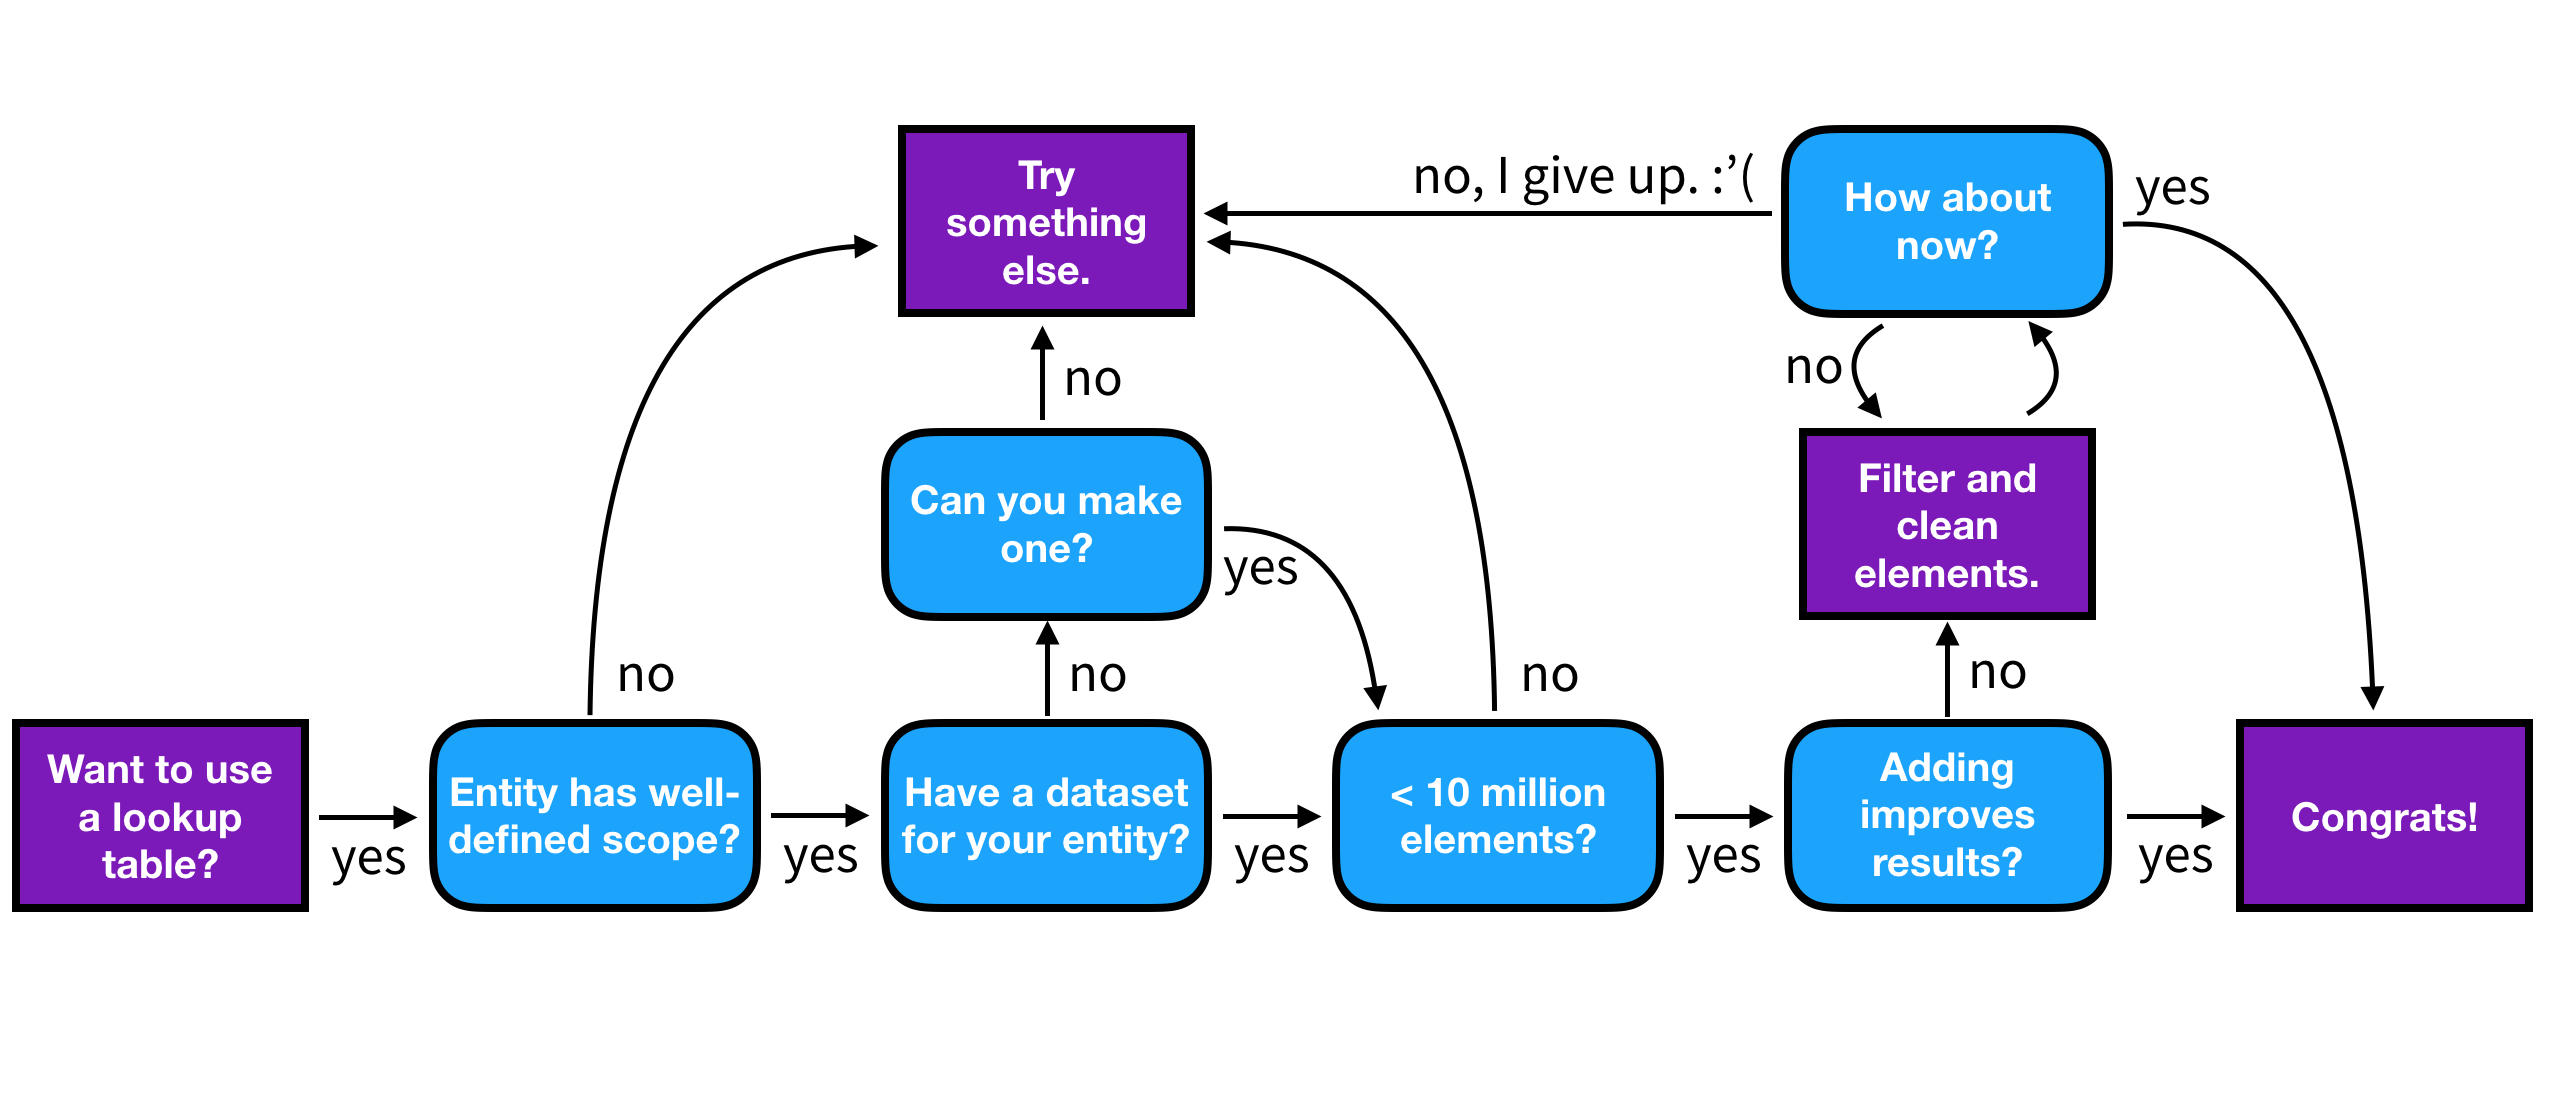
\includegraphics[width=\linewidth,keepaspectratio]{rasa39}
\end{center}
\end{frame}

%%%%%%%%%%%%%%%%%%%%%%%%%%%%%%%%%%%%%%%%%%%%%%%%%%%%%%%%%%%
 \begin{frame}[fragile]\frametitle{Lookups Example}
Create a lookup values file, data/food/food.txt containing several food names

\begin{lstlisting}
mapo tofu
chana masala
sushi
pizza
...
\end{lstlisting}

Add that at the end of nlu.md
\begin{lstlisting}
## lookup:food
   data/food/food.txt
\end{lstlisting}

\end{frame}

%%%%%%%%%%%%%%%%%%%%%%%%%%%%%%%%%%%%%%%%%%%%%%%%%%%%%%%%%%%
 \begin{frame}[fragile]\frametitle{Lookups Training}
Say, one of the examples in your nlu.md is

\begin{lstlisting}
* restaurant_search
	- Could you help me find an [empanada](food) place?

\end{lstlisting}
Train this model using the following configuration in config.yml
\begin{lstlisting}
language: "en"

pipeline:
- name: "nlp_spacy"
- name: "tokenizer_spacy"
- name: "intent_entity_featurizer_regex"
- name: "ner_crf"
  features: [
              ["low", "title", "upper"],
              ["bias", "low", "prefix5", "prefix2", "suffix5", "suffix3",
               "suffix2", "upper", "title", "digit", "pattern"],
              ["low", "title", "upper"]
            ]
\end{lstlisting}

Since tables use regular expressions for matching, we'll need intent\_entity\_featurizer\_regex and the pattern feature in ner\_crf.

\end{frame}

%%%%%%%%%%%%%%%%%%%%%%%%%%%%%%%%%%%%%%%%%%%%%%%%%%%%%%%%%%%
 \begin{frame}[fragile]\frametitle{Lookup Conclusions}
\begin{itemize}
\item Keep them narrow: have a well defined scope
\item Keep them clean: no junk values
\item Keep them short. Giant lookup tables can also add a large amount of time to training
\item Further advancements: Fuzzy match, character n-grams (sub word matching)
\end{itemize}


\end{frame}
